%!TEX root = ../Thesis.tex
\chapter{predictPotency}

A main goal of this thesis has been to use the preclinical data more efficiently. Instead of testing randomly new absorption enhancers or what intuitively seems promising, a model built on previous experiences, can fast systematically evaluate larger libraries of molecules.

Very early in the project three areas to predicts were identified. These were solubility, critical micelle concentration (CMC) and permeation enhancement. In Novo Nordisk for purposes securing intellectual properties, the default rule is that no in-house data generated by the drug development projects can be published. Therefore all data used in this PhD thesis was already public available from third-party sources or conducted in experiments for this thesis only. 

Figure \ref{workSummary} outline the first idea of a workflow in order to select new enhancers. CMC, solubility and permeation potency was identified as important. Data on \textit{in-vitro} Caco-2 permeation enhancement or similar pre-clinical studies were not expected alone to be useful to select new enhancers. As discussed in Section \ref{someWhere} \text{in-vitro} studies tend to overestimate the importance and impact of lipophilicity in absorption enhancers. Enhancers with C16 carbon chains are found 10-50 fold more potent thant their C10 counter parts. Nevertheless  C16 carbon chain based permeation enhancer, have quite dissappoting not delivered the same potency in in vivo studies. An obvious testimony is that no public announced clincal trials using C16 surfactant peptide absorption enhancers \cite{aguirre2016current}. It was noted that in CMC was correlated with high absorption potency, initially to collect data sets on CMC values was a central part. However, during the project I found no evidence that low CMC values directly should cause permeation enhancement, rather CMC simply being one of more collective attributes associated with lipophilicity. Therefore it would make more sense to build predictive models on the attributes that resembled real life absorption the most. Molecular solublity in watery buffers is obviously also negatively associated with lipophilicity/hydrophibicity. In a worst case scenario potency predictions and solubility predictions for given test set of new molecules will be be highly negatively correlated. In such case the collective model will state, predict there is only low potent short chain soluble enhancers or high potent long chain low soluble enhancers. Perhaps some not identified molecular properties will both promote solublity and potency.

Two type of type of data set was obtained from public sources. One data set was obtained in an effort to use text mining to collect examples of compounds being mentiened for being permeation enhancers and/or absorption enhancers. The data set was aquirred by Sten and Sarah Øster Brebbia (cite srah thesis). A list of 167 compounds originating from patent applications and research articles was compiled. It was assumed that surfactant enhancement is a rare property of molecules such that any random molecule would likely not be an enhancer. Random molecules of similar weight was acquired from a (compound DATABASE?). With the software package ACDlabs 49 chemical descriptors was computed for both sets of molecules and linear discriminant analysis has been used to learn a class separation rule to identify typical enhancer like molecules. Although a valid cross-validation of the classification model predicted a nearly perfect prediction accuracy, the model failed in a proof of concept to point of 5 molecules which were tested in-house in the Caco-2 model. The reasons why this approach failed inspite of a promising cross-validation, is likely violation of the IID assumptions, that also machine learning rely on. Introduction to the IID assumptions can be found in Section \ref{blaret}. In machine learning it is central that observations are drawn independently and from identical 

non-idenpendent, because similar molecule got mentioned in same paper
non identical distribution, poisitive enhancer examples were clearly originated from a population of molecules loosly defined at those someone would feel realisticly ever could be a part of a formulation. Thus many fairly rare atoms would not be a part of the molecule. Likewise pharmaceutical excipient tend not to be highly substituted with a mix of random functional groups.


e
\begin{figure}[ht]
\label{workSummary}
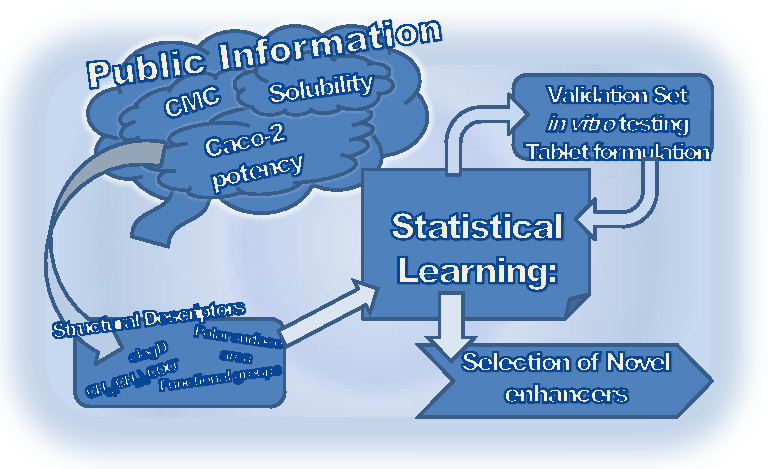
\includegraphics{graphics/workSummary_130mm.pdf}
\caption{Project idea. This figure was first designed for PhD-related presentations given by the author.}
\end{figure}


\begin{figure}[ht]
\label{devel_fassif}
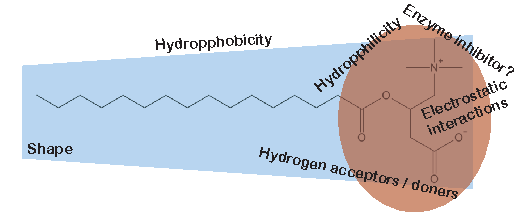
\includegraphics{graphics/typeOfSurfactant.pdf}
\caption{how does a surfactant like enhancer look like. This figure was first designed for PhD-related presentations given by the author.}
\end{figure}

\begin{figure}[ht]
\label{devel_fassif}
\includegraphics[width=\textwidth, height=\textheight, keepaspectratio]{graphics/predictPotencySummary.pdf}
\caption{Outline how to predictions are made. This figure was first designed for PhD-related presentations given by the author.}
\end{figure}

The decision tree ensemble random forest have a series of useful diagnostics which have been used in this thesis work.

\newpage

\includepdf[pages={1-},scale=0.90,pagecommand={\pagestyle{myruled}}]{chapters/predictPotencyArt.pdf}
